\documentclass[a4paper,10pt]{article}
\renewcommand{\baselinestretch}{0.8}
 
\usepackage[svgnames,table,hyperref]{xcolor}
 
\usepackage{titlesec}
\titlespacing{\section}{0pt}{10pt}{5pt}[0pt]
\titlespacing{\subsection}{0pt}{10pt}{5pt}[0pt]
\titlespacing{\subsubsection}{0pt}{5pt}{2pt}[0pt]
\titleformat{\section}{\center}{}{0em}{\MakeUppercase}[\titlerule]
\titleformat{\subsection}{\small}{}{0em}{\MakeUppercase}[\titlerule]
\titleformat{\subsubsection}{\small}{}{0em}{\MakeUppercase}

\newcommand{\uone}[2]{\colorbox{gray}{\textcolor{white}{\parbox{\linewidth-2.4}{\scshape{\medium\textbf{#1}} }}}\\}

\usepackage[landscape]{geometry}
\geometry{
 total={210mm,297mm},
 left=5mm,
 right=5mm,
 top=15mm,
 bottom=0mm,
 }
\usepackage[utf8]{inputenc}
\usepackage[normalem]{ulem}
\usepackage{amssymb}
\usepackage{amsmath}
\usepackage{amsfonts}
\usepackage{multicol}
\usepackage{mathtools}
\usepackage[ngerman]{babel}

\usepackage{enumitem}
\setlist{nolistsep}

\usepackage{fancyhdr}
\pagestyle{fancy}
\fancyhf{}
\rhead{Joshua Näf, \textit{naefjo@ethz.ch}; Franz Bühlmä, \textit{franzbu@ethzch}}
\lhead{\textbf{Dimensionieren 1 HS19 Prof. Dr. Mazza}}
\setlength{\headsep}{1mm}

\usepackage{graphicx}
\graphicspath{ {./images/} }

\setlength\parindent{0pt}


\title{Dimensionieren 1 Zusammenfassung\vspace{-2ex}}
\author{Joshua Näf, naefjo@ethz.ch}
\date{}

\setlength{\columnseprule}{1px}


\begin{document}
\begin{multicols}{3}

%\maketitle
\uone{Methoden d Strukturanalyse}
%\section{Methoden d Strukturanalyse}
    \subsection{Gleichungen des kontinuums:}
        \subsubsection{GGWB des Kontinuums:}
        \[\sigma_{11,1} + \sigma_{12,2} + \sigma_{13,3} + f_1 = 0\]
        \[\sigma_{21,1} + \sigma_{22,2} + \sigma_{23,3} + f_2 = 0\]
        \[\sigma_{31,1} + \sigma_{32,2} + \sigma_{33,3} + f_3 = 0\]
        \subsubsection{Stoffgleichungen (SG):}
        \[\epsilon_{11} = \frac{1}{E}\lbrack\sigma_{11} - \nu(\sigma_{22} + \sigma_{33})\rbrack\]
        \[\epsilon_{22} = \frac{1}{E}\lbrack\sigma_{22} - \nu(\sigma_{11} + \sigma_{33})\rbrack\]
        \[\epsilon_{33} = \frac{1}{E}\lbrack\sigma_{33} - \nu(\sigma_{22} + \sigma_{11})\rbrack\]
        \[\sigma_{11}=\frac{E}{1+\nu}\lbrack\epsilon_{11}+\frac{\nu}{1-2\nu}(\epsilon_{11}+\epsilon_{22}+\epsilon_{33})\rbrack\]
        \[\sigma_{22}=\frac{E}{1+\nu}\lbrack\epsilon_{22}+\frac{\nu}{1-2\nu}(\epsilon_{11}+\epsilon_{22}+\epsilon_{33})\rbrack\]
        \[\sigma_{33}=\frac{E}{1+\nu}\lbrack\epsilon_{33}+\frac{\nu}{1-2\nu}(\epsilon_{11}+\epsilon_{22}+\epsilon_{33})\rbrack\]
        \[\epsilon_{12}=\frac{\tau_{12}}{2G}; \quad 2G=\frac{E}{1+\nu}\]
        \subsubsection{Kinematische Randbedingungen (KR):}
        \[\epsilon_{11} = u_{11}\quad\quad\quad\quad\epsilon_{12} = \frac{1}{2}(u_{12} + u_{21})\]
        \[\epsilon_{22} = u_{22}\quad\quad\quad\quad\epsilon_{13} = \frac{1}{2}(u_{13} + u_{31})\]
        \[\epsilon_{33} = u_{33}\quad\quad\quad\quad\epsilon_{23} = \frac{1}{2}(u_{23} + u_{32})\]
        
\uone{Balken}
%\section{Balken}
    2 Möglichkeiten: Statische Formulierung und Kinematische Formulierung.\\
    Statische Formulierung: GGB \& SG erfüllt, KR zum Teil nicht. Generell zu weich.\\
    Kinematische Formulierung: GGB \& SG nicht erfüllt, KR schon. Steifer als echt. Schlechte approx mit nur einer Funktion. Approximation wird besser durch besseren Ansatz und mehrere Elemente.
    \subsection{Energiesätze:}
        \subsubsection{Definitionen:}
            \begin{itemize}
                \item Spannungsfeld $\sigma_{ij}(x,y,z)$ zulässig falls: GGB \& \textit{stat} RB erfüllt.
                \item Verschiebungsfeld $u_i(x,y,z)$ zulässig falls: stetig \& \textit{kin} RB erfüllt (schwächere Bedingung).
                \item Verschiebungsfeld \& Spannungsfeld verträglich iff SG erfüllt.
                \item Deformationsenergie: $\displaystyle U=\frac{1}{2}\iiint_V \sigma_{ij}\epsilon_{ij}dV$
                \item Potential äussere Energie:\\
                $\displaystyle V=-\iiint_V f_iu_idV-\sum_{a}\underline{F_a}\cdot\underline{u_a}$ 
                \item Potentielle Energie: $E_p=U+V$
                \item Komplementäre Deformationsenergie:\\ $U_K=\iiint_V(\oint_0^{\sigma_{ij}}\epsilon_{ij}d\sigma_{ij})dV := U$  (lin. elast.)
            \end{itemize}
        \subsubsection{Satz vom Minium der potentiellen Energie (SMPE):}
            Aus der Menge der zulässigen Verschiebungsfelder $u_i^*(x,y,z)$ \& der damit verträglichen Spannungsfelder $\sigma_{ij}^*(x,y,z)$ macht das wirkliche Verschiebungsfeld $u_i(x,y,z)$ $E_P$ minimal. $E_p(u_i) < E_p(u_i^*)$\\\\
            \textit{Direkte Anwendung:} Ansatz für $u_i(x,y,z,a_\gamma)$, zulässig (stetig, KRB erfüllt). Berchene $\epsilon_{ij}^*$ (aus KR) und verträgliche Spannungen $\sigma_{ij}^*$ (aus SG). $\sigma_{ij}^*$ braucht nicht zulässig zu sein (GGB \& SRB evtl. nicht erfüllt). Berechne $E_p(u_i^*)$ und bestimme $a_\gamma$ mit $\frac{\partial E_p}{\partial a_\gamma}=0$.
        \subsubsection{Satz vom Minimum der komplementären Deformationsenergie (SMkDE):}
            Aus der Menge der zulässigen Spannungsfelder $\sigma_{ij}^*(x,y,z)$ \& damit verträglichen $\epsilon_{ij}^*(x,y,z)$ macht das wirkliche Spannungsfeld $\sigma_{ij}(x,y,z)$ die komplementäre Deformationsenergie $U_K$ minimal. $U_K(\sigma_{ij}) < U_K(\sigma_{ij}^*)$\\\\
            \textit{Direkte Anwendung:} Ansatz für $\sigma_{ij}^*(x,y,z,a_\gamma)$, zulässig (GGB, SRB erfüllt). Berechne $\epsilon_{ij}^*$ (aus SG), nicht unbedingt zulässig (KR, KRB eventuell nicht erfüllt). Berechne $U_K(\sigma_{ij}^*)$ und bestimme $a_\gamma$ mit $\frac{\partial U}{\partial a_\gamma}=0$.
        \subsubsection{Bsp:}
            Ansatz:\\
            $u_y=ax^3+bx^2; u_x=-\frac{du_y}{dx}y= -(3ax^2+2bx)y; u_z = 0$\\
            KR: $\epsilon_{xx} =(-6ax-2b)y$; $\epsilon_{yy}=\epsilon_{zz}=\epsilon_{xy}=\epsilon_{yz} = \epsilon_{xz}=0$\\
            SG: $\sigma_{xx} = \alpha(-6ax-3b)y$, $\sigma_{xy}=\sigma_{xz}=\sigma_{yz}=0$\\ $\sigma_{yy}=\sigma_{zz}=2G\frac{\nu}{1-2\nu}(-6ax-2b)y$\\
            SMPE:\\
            $U=\frac{1}{2}\int_0^l\int_\frac{-h}{2}^\frac{h}{2}\int_{-\frac{b}{2}}^\frac{b}{2}(\sigma_{xx}\cdot\epsilon_{xx})dzdydx=6\cdot\alpha\cdot I\cdot l(\alpha^2l^2+\frac{b^2}{3}+abl)$\\
            $V=-P\cdot u_y(x=l)=-P(al^3+bl^2)$\\
            $E_p=6\alpha Il(a^2l2+\frac{b^2}{3}+abl)-P(al^3+bl^2)$
            \[\frac{\partial E_p}{\partial a} = 0 \Rightarrow a=-\frac{P}{6\alpha I};\quad\frac{\partial E_p}{\partial b} = 0 \Rightarrow b=-\frac{P}{2\alpha I}\]
        \subsubsection{SMPE \& FEM:}
            Relation der Verschiebungsfreiheitsgrade der Knoten ($\{u\}$) und äusseren Kräften an den Knoten ($\{F\}$) über die globale Steifigkeitsmatrix ($\{K\}\in\mathbb{R}^{6\times6}$): $\{F\}=\{K\}\{u\}$
            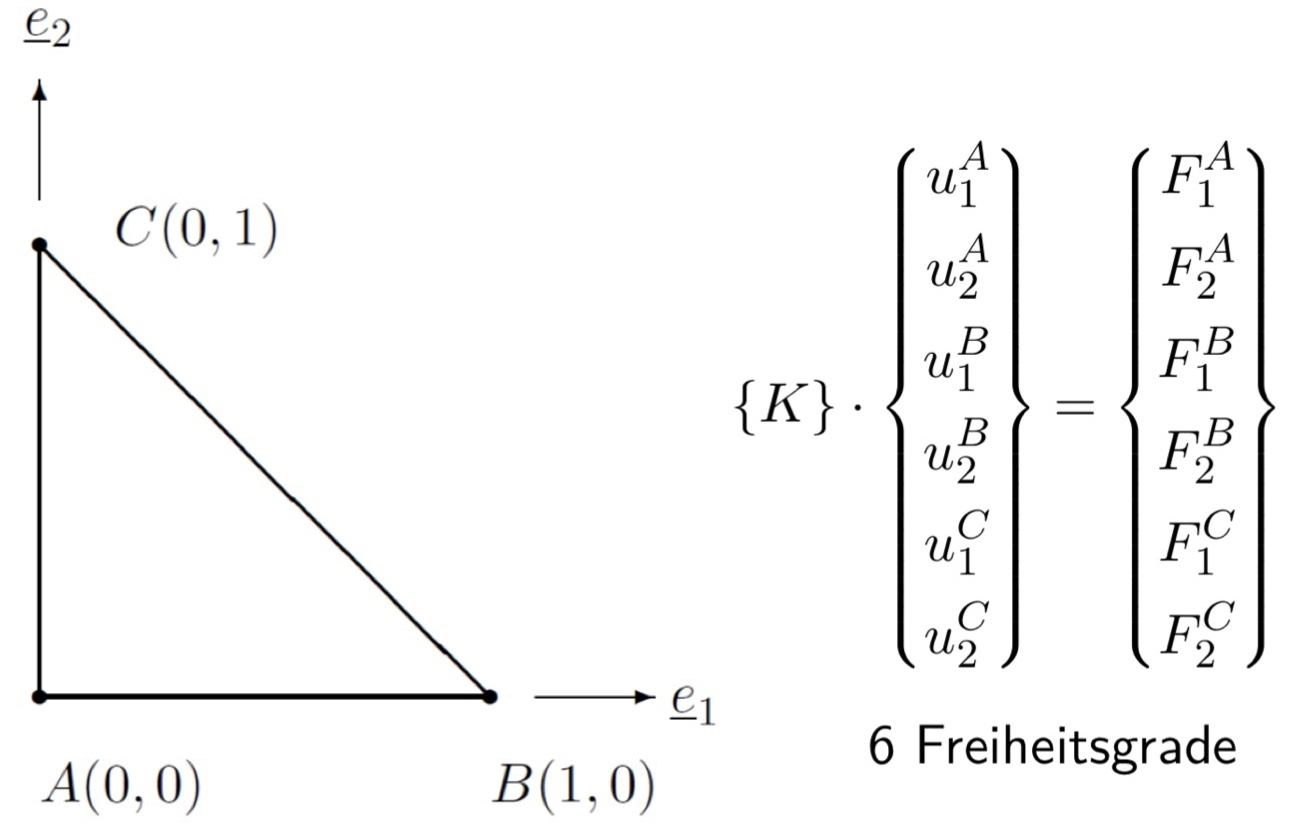
\includegraphics[width=70mm]{Dreieckselement}
        \subsubsection{Bsp}
            $u_1=ax_1+bx_2+c$; $u_2=dx_1+ex_2+f$\\
            $\Rightarrow u_1(x_1=0,x_2=0)=u_1^A$; $u_2(x_1=0,x_2=0)=u_2^A$;...\\
            $\Rightarrow u_1=(u_1^B-u_1^A)x_1+(u_1^C-u_1^A)x_2+u_1^A$;\\
            $u_2=(u_2^B-u_2^A)x_1+(u_2^C-u_2^A)x_2+u_2^A$\\
            KR:\\
            $\epsilon_{11}=(u_1^B-u_1^A)$; $\epsilon_{22}=(u_2^C-u_2^A)$; $\epsilon_{12}=\frac{1}{2}(u_2^B-u_2^A+u_1^C-u_1^A)$
            $\Rightarrow\sigma_{ij}(u_1^A,...,u_2^C,E,\nu)$\\
            $U=\frac{1}{2}\cdot\frac{1}{2}(\sigma_{11}\cdot\epsilon_{11}+\sigma_{22}\cdot\epsilon_{22}+2\sigma_{12}\cdot\epsilon_{12})\cdot t$ mit Dicke $t$ und Fläche $\frac{1}{2}$.\\
            $V=-(F_1^A\cdot u_1^A+F_2^A\cdot u_2^A+...+F_2^C\cdot u_2^C$\\
            $E_p=U+V=E_p(u_1^A,...,u_2^C,E,\nu,t)=\alpha_1(u_1^A)^2+\alpha_2u_1^Au_1^B+ ...-(F_1^Au_1^A+...)$\\
            Minimum $E_p:$ $\frac{\partial E_p}{\partial u_i^\kappa}=0$ mit $i=1,2$ \& $\kappa=A,B,C$ (6Gl)\\
            Bsp: $\frac{\partial E_p}{\partial u_1^A}=\frac{\partial U}{\partial u_1^A}+\frac{\partial V}{\partial u_1^A}$ (lin. Fkt. in $u_1^A,..,u_2^C$) \\$\Rightarrow F_1=\kappa_{11}u_1^A+...+\kappa_{16}u_2^c$; $\kappa_{11},...,\kappa_{16}$: 1. Zeile von $\{K\}$

\uone{Scheibe}
%\section{Scheibe}
    \subsection{Definition:}
        Scheibenelement: Dünnwandige Struktur mit Belastung in der Ebene. Äussere Kräfte dargestellt durch $N_x,N_y,N_{xy},N_{yx}$: Kräfte pro Längeneinheit ($\rightarrow$ Spannungen $\sigma_{xx},\sigma_{yy},\tau_{xy}$ über Dicke t integriert).
        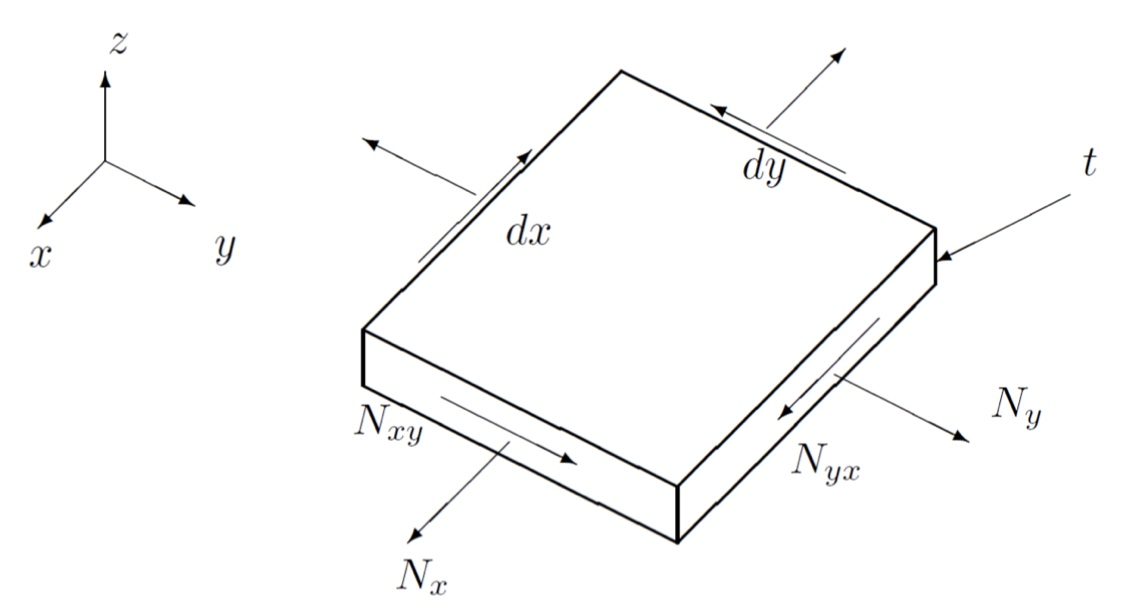
\includegraphics[width=50mm]{Balkenelement.jpeg}
    \subsection{Annahmen:}
        \begin{enumerate}[noitemsep]
            \item Ebener Spannungszustand ($\sigma_{zz},\tau_{xz},\tau_{yz}=0$)
            \item Übrige Spannungskomponenten sind konstant verteilt in z-Richtung (homogene Spannungsverteilung)
            \item Keine Volumenkräfte
        \end{enumerate}
        1.,2.: Vernünftig, weil planare Dimensionen $\gg$ t \& keine Biegung. GGB reduziert sich zu:
        \[\sigma_{xx,x} + \tau_{xy,y}=0\quad\quad\sigma_{yy,y} + \tau_{xy,x}=0\]
        Definiere $F(x,y)$ (ayrische Spannungsfkt) mit $\sigma_{xx}=F_{,yy}$; $\sigma_{yy}=F_{,xx}$; $\tau_{xy}=-F_{,xy}$. Aus Kompatibilitätsbedingung: $\epsilon_{xx,yy}+\epsilon_{yy,xx}=2\epsilon_{xy,xy} \rightarrow \Delta\Delta F=0$ (Bi-potential Gleichung) Funktion F(x,y) so wählen, damit RB erfüllt.
    \subsection{Scheibe mit Loch:}
        Annahmen:
        \begin{itemize}
            \item Lochradius a $\ll$ L
            \item Belastung durch uniforme, einachsige Spannung S in grosser Entfernung vom Loch
        \end{itemize}
        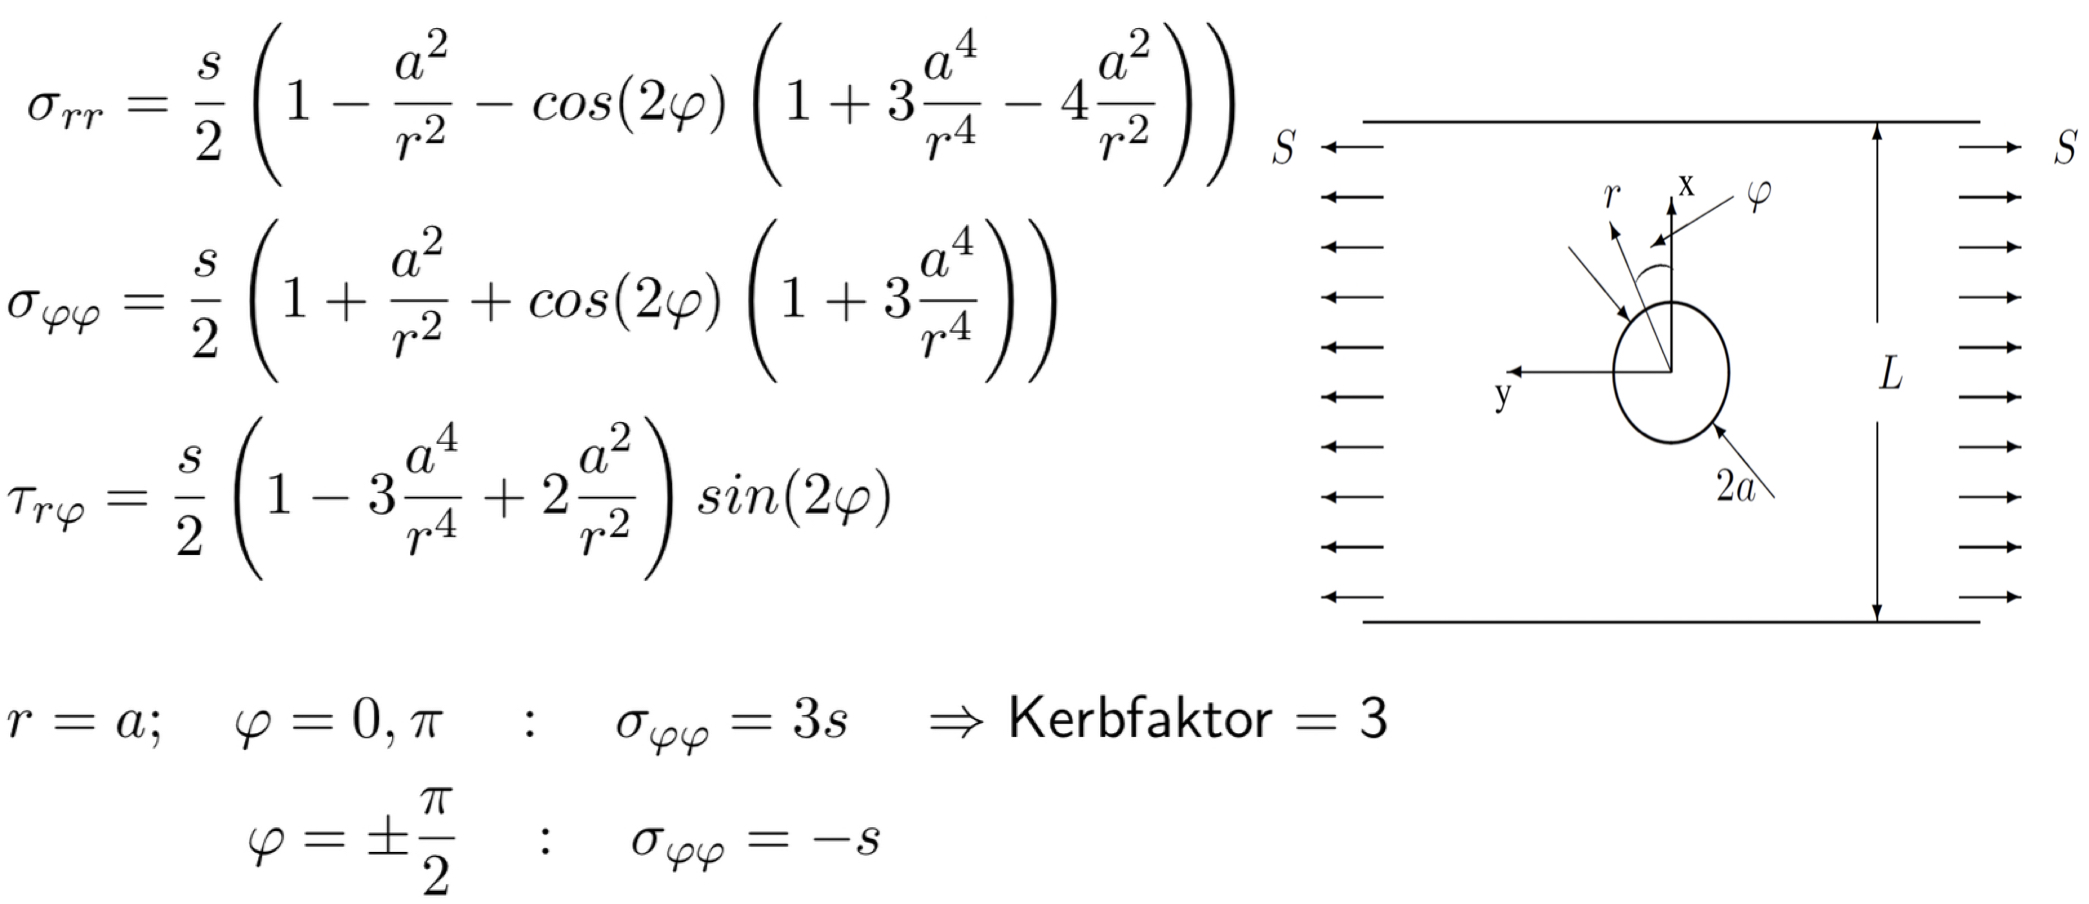
\includegraphics[width=90mm]{Scheibeloch}
        Superposition von mehreren Spannungen \& Spannungsrichtungen möglich. Bei Schubspannungen in Hauptspannungen umwandlen (Mohrscher Kreis).
    \subsection{Scheibe mit Riss:}
        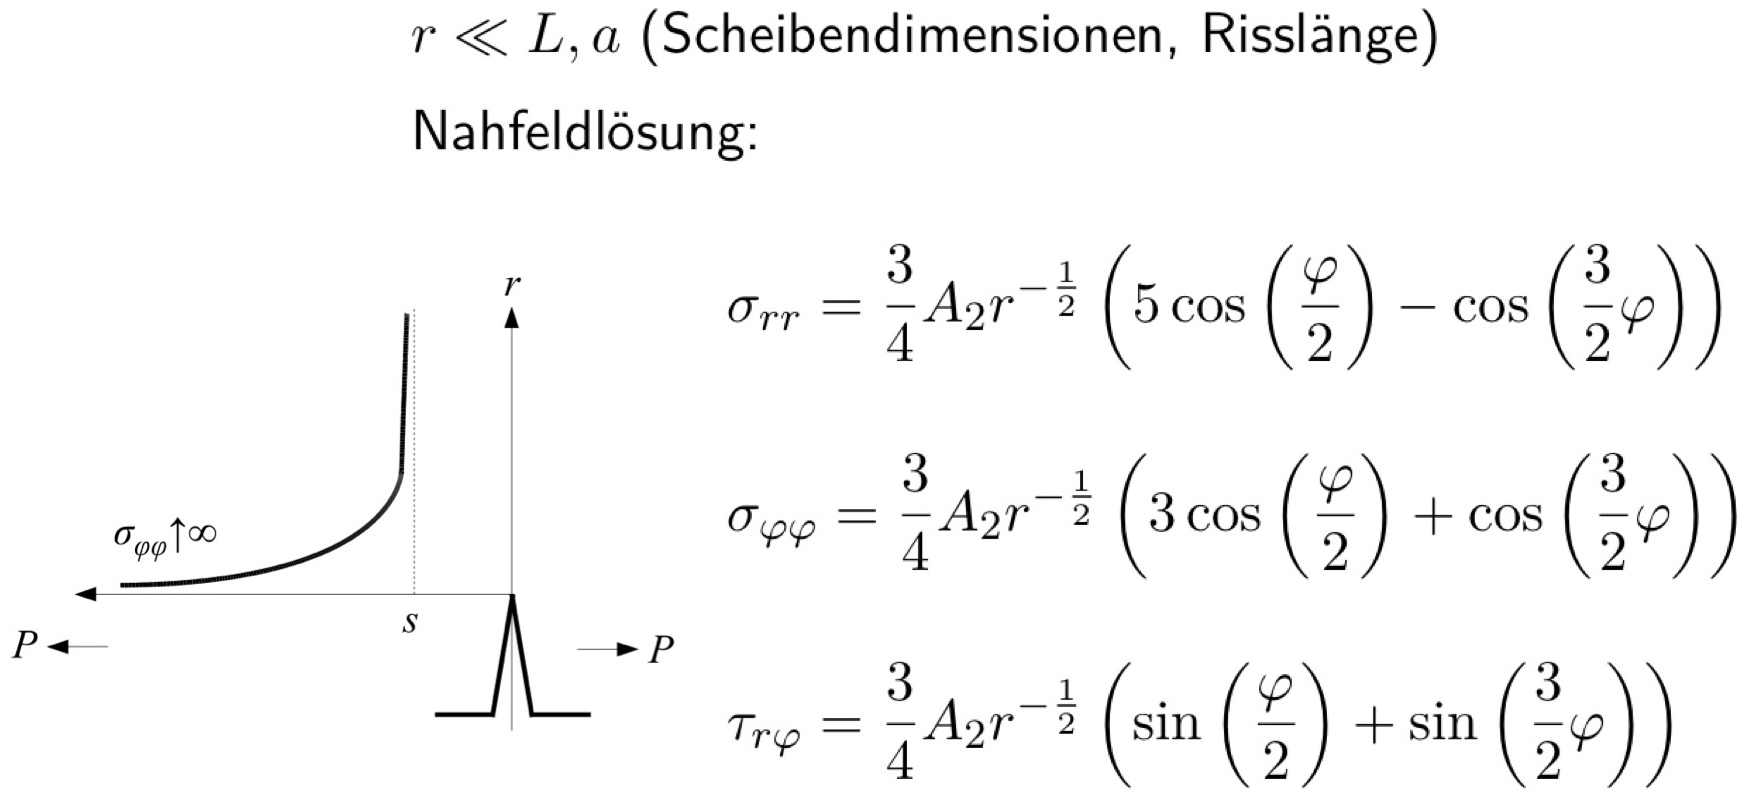
\includegraphics[width=80mm]{Scheiberiss}
        
\uone{Materialverhalten}
%\section{Materialverhalten}
    \subsection{Festigkeitshypothesen:}
        \subsubsection{Fliessbedingung:}
            Fliessfunktion: $\Phi(\sigma)$\\
            Fliessbedingung: $\Phi(\sigma)<0$ (elastisch), $\Phi(\sigma)=0$ (plastisch)
            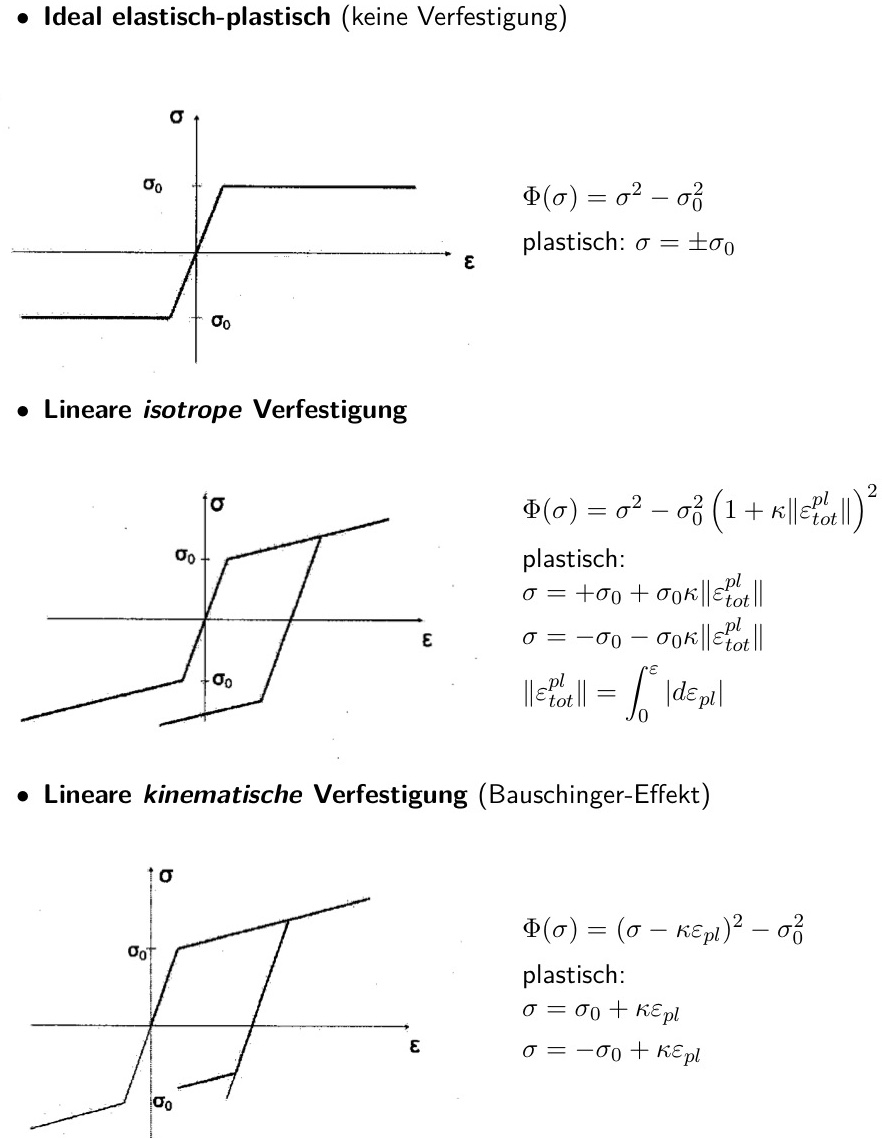
\includegraphics[width=70mm]{images/Fliessbedingungen.jpeg}
        \subsubsection{von Mieses'sche Vergleichsspannung:}
            \[\Phi_{v.Mises}= \sigma_1^2+\sigma_2^2+\sigma_3^2-\sigma_1\sigma_2-\sigma_1\sigma_3-\sigma_2\sigma_3 -\sigma_0^2\quad(=0)\]
            \[\Leftrightarrow \sigma_{v. Mises}^{vgl}= \sqrt{\sigma_1^2+\sigma_2^2+\sigma_3^2-\sigma_1\sigma_2-\sigma_1\sigma_3-\sigma_2\sigma_3} \quad\textrm(HS)\]
        \subsubsection{Tresca'sche Vergleichsspannung:}
            Konservativer als von Mises'sche Vergleichsspannung (Grenzfläche von Sechseck schneller erreicht als von Ellipse).
            \[\frac{1}{2}Max(|\sigma_1-\sigma_2|,|\sigma_2-\sigma_3|,|\sigma_3-\sigma_1|)=\tau_0=\frac{\sigma_0}{2}\]

\end{multicols}
\end{document}